% !TEX TS-program = pdflatex
% !TEX encoding = UTF-8 Unicode
\documentclass[border=0mm]{standalone}
% packages
\usepackage{tikz}
\usetikzlibrary{patterns}
\usepackage{amsmath,amssymb}
\usepackage{bm}
\usepackage{pgfplots}
\pgfplotsset{compat=1.15}
% start document
\begin{document}
% generated by ROOT (CERN)
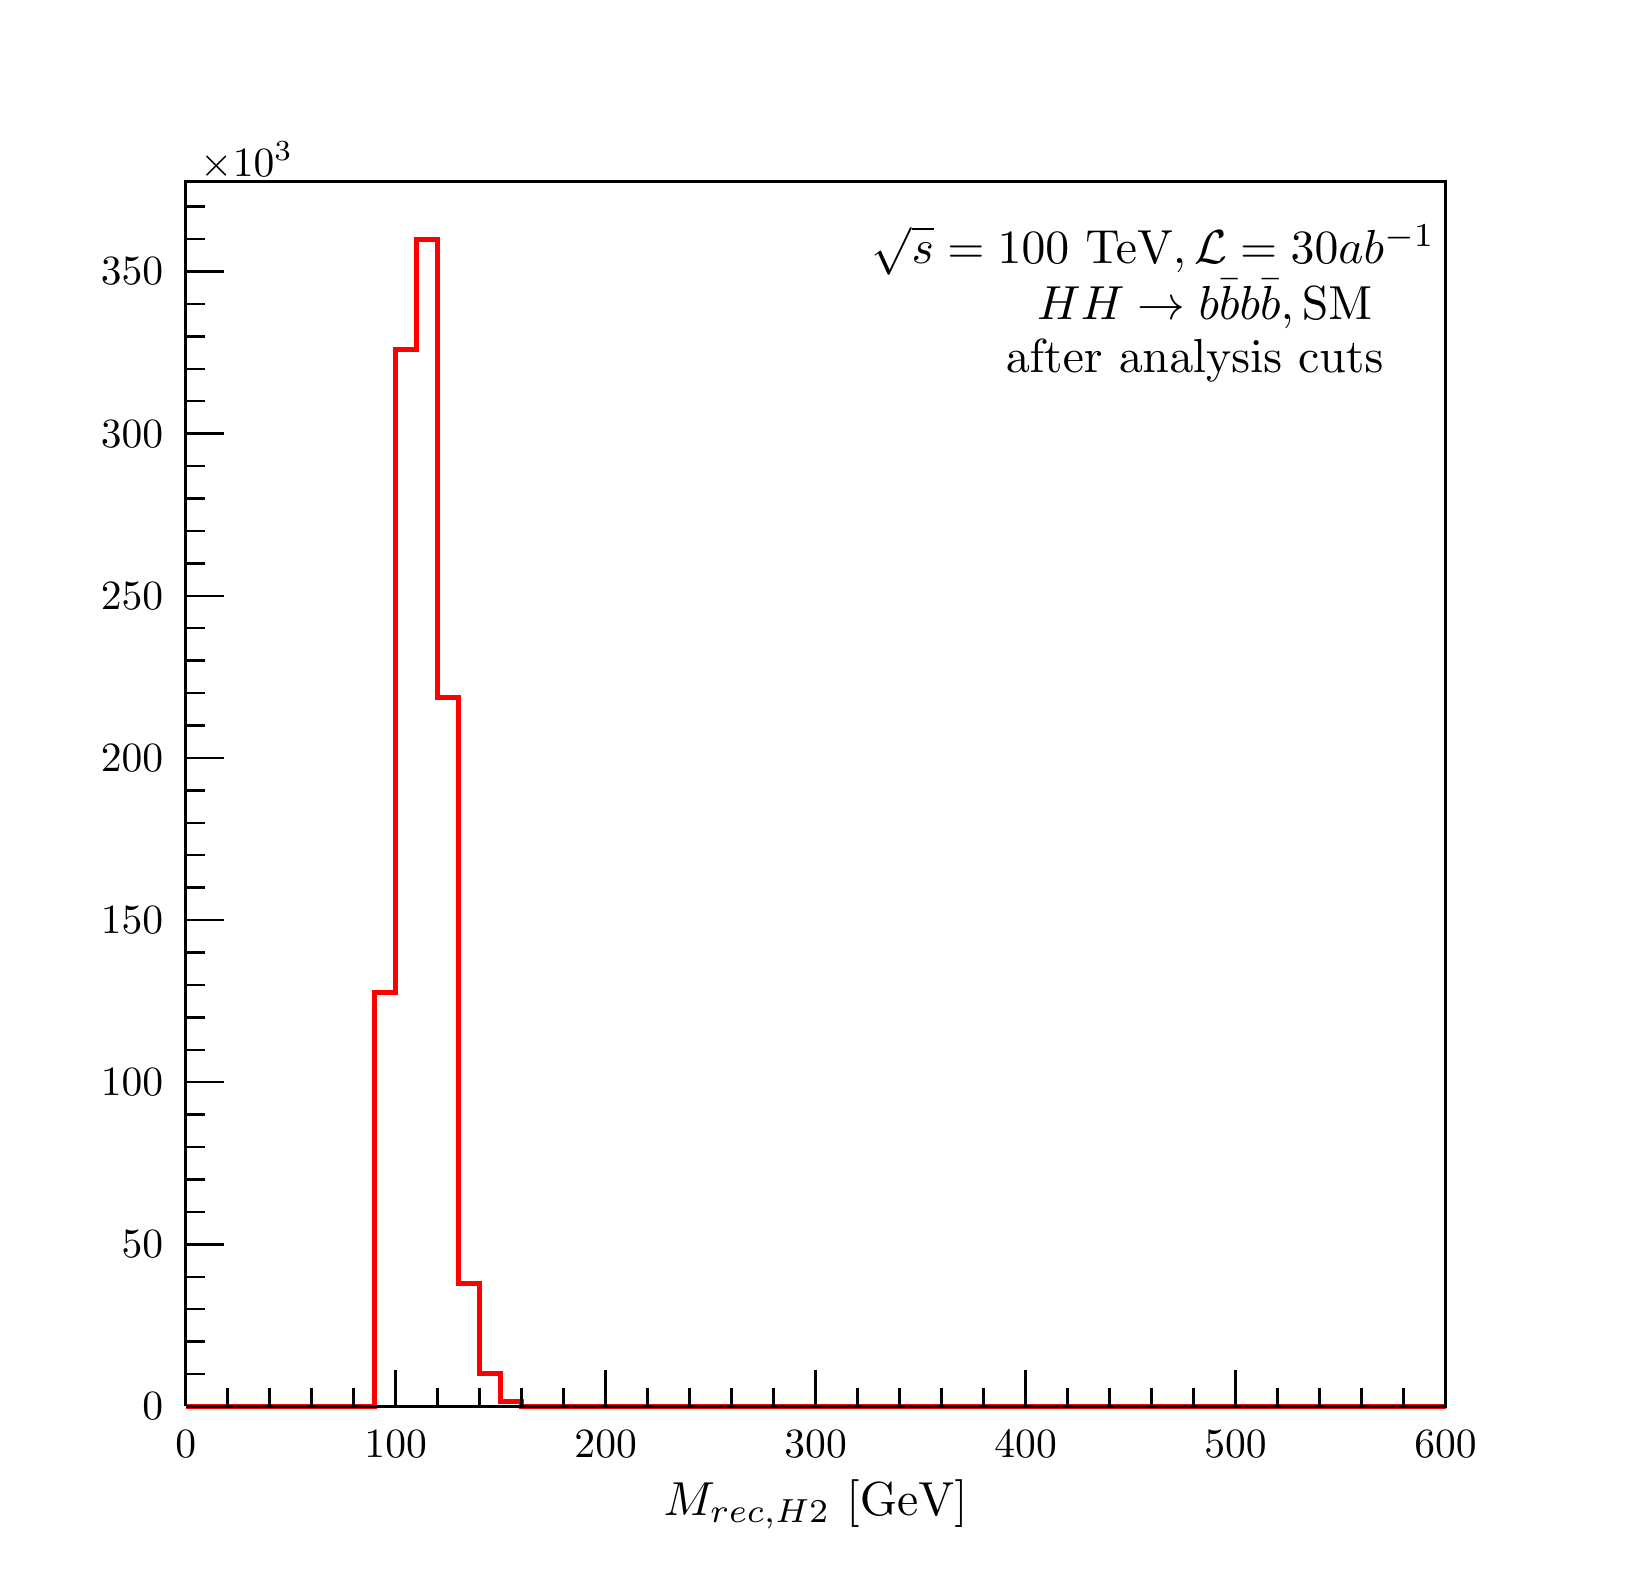
\begin{tikzpicture}
\pgfdeclareplotmark{cross} {
\pgfpathmoveto{\pgfpoint{-0.3\pgfplotmarksize}{\pgfplotmarksize}}
\pgfpathlineto{\pgfpoint{+0.3\pgfplotmarksize}{\pgfplotmarksize}}
\pgfpathlineto{\pgfpoint{+0.3\pgfplotmarksize}{0.3\pgfplotmarksize}}
\pgfpathlineto{\pgfpoint{+1\pgfplotmarksize}{0.3\pgfplotmarksize}}
\pgfpathlineto{\pgfpoint{+1\pgfplotmarksize}{-0.3\pgfplotmarksize}}
\pgfpathlineto{\pgfpoint{+0.3\pgfplotmarksize}{-0.3\pgfplotmarksize}}
\pgfpathlineto{\pgfpoint{+0.3\pgfplotmarksize}{-1.\pgfplotmarksize}}
\pgfpathlineto{\pgfpoint{-0.3\pgfplotmarksize}{-1.\pgfplotmarksize}}
\pgfpathlineto{\pgfpoint{-0.3\pgfplotmarksize}{-0.3\pgfplotmarksize}}
\pgfpathlineto{\pgfpoint{-1.\pgfplotmarksize}{-0.3\pgfplotmarksize}}
\pgfpathlineto{\pgfpoint{-1.\pgfplotmarksize}{0.3\pgfplotmarksize}}
\pgfpathlineto{\pgfpoint{-0.3\pgfplotmarksize}{0.3\pgfplotmarksize}}
\pgfpathclose
\pgfusepathqstroke
}
\pgfdeclareplotmark{cross*} {
\pgfpathmoveto{\pgfpoint{-0.3\pgfplotmarksize}{\pgfplotmarksize}}
\pgfpathlineto{\pgfpoint{+0.3\pgfplotmarksize}{\pgfplotmarksize}}
\pgfpathlineto{\pgfpoint{+0.3\pgfplotmarksize}{0.3\pgfplotmarksize}}
\pgfpathlineto{\pgfpoint{+1\pgfplotmarksize}{0.3\pgfplotmarksize}}
\pgfpathlineto{\pgfpoint{+1\pgfplotmarksize}{-0.3\pgfplotmarksize}}
\pgfpathlineto{\pgfpoint{+0.3\pgfplotmarksize}{-0.3\pgfplotmarksize}}
\pgfpathlineto{\pgfpoint{+0.3\pgfplotmarksize}{-1.\pgfplotmarksize}}
\pgfpathlineto{\pgfpoint{-0.3\pgfplotmarksize}{-1.\pgfplotmarksize}}
\pgfpathlineto{\pgfpoint{-0.3\pgfplotmarksize}{-0.3\pgfplotmarksize}}
\pgfpathlineto{\pgfpoint{-1.\pgfplotmarksize}{-0.3\pgfplotmarksize}}
\pgfpathlineto{\pgfpoint{-1.\pgfplotmarksize}{0.3\pgfplotmarksize}}
\pgfpathlineto{\pgfpoint{-0.3\pgfplotmarksize}{0.3\pgfplotmarksize}}
\pgfpathclose
\pgfusepathqfillstroke
}
\pgfdeclareplotmark{newstar} {
\pgfpathmoveto{\pgfqpoint{0pt}{\pgfplotmarksize}}
\pgfpathlineto{\pgfqpointpolar{44}{0.5\pgfplotmarksize}}
\pgfpathlineto{\pgfqpointpolar{18}{\pgfplotmarksize}}
\pgfpathlineto{\pgfqpointpolar{-20}{0.5\pgfplotmarksize}}
\pgfpathlineto{\pgfqpointpolar{-54}{\pgfplotmarksize}}
\pgfpathlineto{\pgfqpointpolar{-90}{0.5\pgfplotmarksize}}
\pgfpathlineto{\pgfqpointpolar{234}{\pgfplotmarksize}}
\pgfpathlineto{\pgfqpointpolar{198}{0.5\pgfplotmarksize}}
\pgfpathlineto{\pgfqpointpolar{162}{\pgfplotmarksize}}
\pgfpathlineto{\pgfqpointpolar{134}{0.5\pgfplotmarksize}}
\pgfpathclose
\pgfusepathqstroke
}
\pgfdeclareplotmark{newstar*} {
\pgfpathmoveto{\pgfqpoint{0pt}{\pgfplotmarksize}}
\pgfpathlineto{\pgfqpointpolar{44}{0.5\pgfplotmarksize}}
\pgfpathlineto{\pgfqpointpolar{18}{\pgfplotmarksize}}
\pgfpathlineto{\pgfqpointpolar{-20}{0.5\pgfplotmarksize}}
\pgfpathlineto{\pgfqpointpolar{-54}{\pgfplotmarksize}}
\pgfpathlineto{\pgfqpointpolar{-90}{0.5\pgfplotmarksize}}
\pgfpathlineto{\pgfqpointpolar{234}{\pgfplotmarksize}}
\pgfpathlineto{\pgfqpointpolar{198}{0.5\pgfplotmarksize}}
\pgfpathlineto{\pgfqpointpolar{162}{\pgfplotmarksize}}
\pgfpathlineto{\pgfqpointpolar{134}{0.5\pgfplotmarksize}}
\pgfpathclose
\pgfusepathqfillstroke
}
\definecolor{c}{rgb}{1,1,1};
\draw [color=c, fill=c] (0,0) rectangle (20,19.4486);
\draw [color=c, fill=c] (0,0) rectangle (20,19.4486);
\draw [color=c, fill=c] (2,1.94486) rectangle (18,17.5038);
\definecolor{c}{rgb}{0,0,0};
\draw [c,line width=0.9] (2,1.94486) -- (2,17.5038) -- (18,17.5038) -- (18,1.94486) -- (2,1.94486);
\definecolor{c}{rgb}{1,1,1};
\draw [color=c, fill=c] (2,1.94486) rectangle (18,17.5038);
\definecolor{c}{rgb}{0,0,0};
\draw [c,line width=0.9] (2,1.94486) -- (2,17.5038) -- (18,17.5038) -- (18,1.94486) -- (2,1.94486);
\definecolor{c}{rgb}{1,0,0};
\draw [c,line width=1.8] (2,1.94486) -- (2.26667,1.94486) -- (2.26667,1.94486) -- (2.53333,1.94486) -- (2.53333,1.94486) -- (2.8,1.94486) -- (2.8,1.94486) -- (3.06667,1.94486) -- (3.06667,1.94486) -- (3.33333,1.94486) -- (3.33333,1.94486) --
 (3.6,1.94486) -- (3.6,1.94486) -- (3.86667,1.94486) -- (3.86667,1.94486) -- (4.13333,1.94486) -- (4.13333,1.94486) -- (4.4,1.94486) -- (4.4,7.19689) -- (4.66667,7.19689) -- (4.66667,15.3741) -- (4.93333,15.3741) -- (4.93333,16.7629) -- (5.2,16.7629)
 -- (5.2,10.9523) -- (5.46667,10.9523) -- (5.46667,3.50765) -- (5.73333,3.50765) -- (5.73333,2.36303) -- (6,2.36303) -- (6,2.00998) -- (6.26667,2.00998) -- (6.26667,1.94486) -- (6.53333,1.94486) -- (6.53333,1.94486) -- (6.8,1.94486) -- (6.8,1.94486)
 -- (7.06667,1.94486) -- (7.06667,1.94486) -- (7.33333,1.94486) -- (7.33333,1.94486) -- (7.6,1.94486) -- (7.6,1.94486) -- (7.86667,1.94486) -- (7.86667,1.94486) -- (8.13333,1.94486) -- (8.13333,1.94486) -- (8.4,1.94486) -- (8.4,1.94486) --
 (8.66667,1.94486) -- (8.66667,1.94486) -- (8.93333,1.94486) -- (8.93333,1.94486) -- (9.2,1.94486) -- (9.2,1.94486) -- (9.46667,1.94486) -- (9.46667,1.94486) -- (9.73333,1.94486) -- (9.73333,1.94486) -- (10,1.94486) -- (10,1.94486) --
 (10.2667,1.94486) -- (10.2667,1.94486) -- (10.5333,1.94486) -- (10.5333,1.94486) -- (10.8,1.94486) -- (10.8,1.94486) -- (11.0667,1.94486) -- (11.0667,1.94486) -- (11.3333,1.94486) -- (11.3333,1.94486) -- (11.6,1.94486) -- (11.6,1.94486) --
 (11.8667,1.94486) -- (11.8667,1.94486) -- (12.1333,1.94486) -- (12.1333,1.94486) -- (12.4,1.94486) -- (12.4,1.94486) -- (12.6667,1.94486) -- (12.6667,1.94486) -- (12.9333,1.94486) -- (12.9333,1.94486) -- (13.2,1.94486) -- (13.2,1.94486) --
 (13.4667,1.94486) -- (13.4667,1.94486) -- (13.7333,1.94486) -- (13.7333,1.94486) -- (14,1.94486) -- (14,1.94486) -- (14.2667,1.94486) -- (14.2667,1.94486) -- (14.5333,1.94486) -- (14.5333,1.94486) -- (14.8,1.94486) -- (14.8,1.94486) --
 (15.0667,1.94486) -- (15.0667,1.94486) -- (15.3333,1.94486) -- (15.3333,1.94486) -- (15.6,1.94486) -- (15.6,1.94486) -- (15.8667,1.94486) -- (15.8667,1.94486) -- (16.1333,1.94486) -- (16.1333,1.94486) -- (16.4,1.94486) -- (16.4,1.94486) --
 (16.6667,1.94486) -- (16.6667,1.94486) -- (16.9333,1.94486) -- (16.9333,1.94486) -- (17.2,1.94486) -- (17.2,1.94486) -- (17.4667,1.94486) -- (17.4667,1.94486) -- (17.7333,1.94486) -- (17.7333,1.94486) -- (18,1.94486);
\definecolor{c}{rgb}{0,0,0};
\draw [c,line width=0.9] (2,1.94486) -- (18,1.94486);
\draw [c,line width=0.9] (2,2.41163) -- (2,1.94486);
\draw [c,line width=0.9] (2.53333,2.17825) -- (2.53333,1.94486);
\draw [c,line width=0.9] (3.06667,2.17825) -- (3.06667,1.94486);
\draw [c,line width=0.9] (3.6,2.17825) -- (3.6,1.94486);
\draw [c,line width=0.9] (4.13333,2.17825) -- (4.13333,1.94486);
\draw [c,line width=0.9] (4.66667,2.41163) -- (4.66667,1.94486);
\draw [c,line width=0.9] (5.2,2.17825) -- (5.2,1.94486);
\draw [c,line width=0.9] (5.73333,2.17825) -- (5.73333,1.94486);
\draw [c,line width=0.9] (6.26667,2.17825) -- (6.26667,1.94486);
\draw [c,line width=0.9] (6.8,2.17825) -- (6.8,1.94486);
\draw [c,line width=0.9] (7.33333,2.41163) -- (7.33333,1.94486);
\draw [c,line width=0.9] (7.86667,2.17825) -- (7.86667,1.94486);
\draw [c,line width=0.9] (8.4,2.17825) -- (8.4,1.94486);
\draw [c,line width=0.9] (8.93333,2.17825) -- (8.93333,1.94486);
\draw [c,line width=0.9] (9.46667,2.17825) -- (9.46667,1.94486);
\draw [c,line width=0.9] (10,2.41163) -- (10,1.94486);
\draw [c,line width=0.9] (10.5333,2.17825) -- (10.5333,1.94486);
\draw [c,line width=0.9] (11.0667,2.17825) -- (11.0667,1.94486);
\draw [c,line width=0.9] (11.6,2.17825) -- (11.6,1.94486);
\draw [c,line width=0.9] (12.1333,2.17825) -- (12.1333,1.94486);
\draw [c,line width=0.9] (12.6667,2.41163) -- (12.6667,1.94486);
\draw [c,line width=0.9] (13.2,2.17825) -- (13.2,1.94486);
\draw [c,line width=0.9] (13.7333,2.17825) -- (13.7333,1.94486);
\draw [c,line width=0.9] (14.2667,2.17825) -- (14.2667,1.94486);
\draw [c,line width=0.9] (14.8,2.17825) -- (14.8,1.94486);
\draw [c,line width=0.9] (15.3333,2.41163) -- (15.3333,1.94486);
\draw [c,line width=0.9] (15.8667,2.17825) -- (15.8667,1.94486);
\draw [c,line width=0.9] (16.4,2.17825) -- (16.4,1.94486);
\draw [c,line width=0.9] (16.9333,2.17825) -- (16.9333,1.94486);
\draw [c,line width=0.9] (17.4667,2.17825) -- (17.4667,1.94486);
\draw [c,line width=0.9] (18,2.41163) -- (18,1.94486);
\draw [anchor=base] (2,1.30306) node[scale=1.50291, color=c, rotate=0]{0};
\draw [anchor=base] (4.66667,1.30306) node[scale=1.50291, color=c, rotate=0]{100};
\draw [anchor=base] (7.33333,1.30306) node[scale=1.50291, color=c, rotate=0]{200};
\draw [anchor=base] (10,1.30306) node[scale=1.50291, color=c, rotate=0]{300};
\draw [anchor=base] (12.6667,1.30306) node[scale=1.50291, color=c, rotate=0]{400};
\draw [anchor=base] (15.3333,1.30306) node[scale=1.50291, color=c, rotate=0]{500};
\draw [anchor=base] (18,1.30306) node[scale=1.50291, color=c, rotate=0]{600};
\draw (10,0.700151) node[scale=1.72557, color=c, rotate=0]{$M_{rec, H2} ~[\text{GeV}]$};
\draw [c,line width=0.9] (2,1.94486) -- (2,17.5038);
\draw [c,line width=0.9] (2.48,1.94486) -- (2,1.94486);
\draw [c,line width=0.9] (2.24,2.35669) -- (2,2.35669);
\draw [c,line width=0.9] (2.24,2.76853) -- (2,2.76853);
\draw [c,line width=0.9] (2.24,3.18036) -- (2,3.18036);
\draw [c,line width=0.9] (2.24,3.59219) -- (2,3.59219);
\draw [c,line width=0.9] (2.48,4.00402) -- (2,4.00402);
\draw [c,line width=0.9] (2.24,4.41585) -- (2,4.41585);
\draw [c,line width=0.9] (2.24,4.82769) -- (2,4.82769);
\draw [c,line width=0.9] (2.24,5.23952) -- (2,5.23952);
\draw [c,line width=0.9] (2.24,5.65135) -- (2,5.65135);
\draw [c,line width=0.9] (2.48,6.06318) -- (2,6.06318);
\draw [c,line width=0.9] (2.24,6.47502) -- (2,6.47502);
\draw [c,line width=0.9] (2.24,6.88685) -- (2,6.88685);
\draw [c,line width=0.9] (2.24,7.29868) -- (2,7.29868);
\draw [c,line width=0.9] (2.24,7.71051) -- (2,7.71051);
\draw [c,line width=0.9] (2.48,8.12234) -- (2,8.12234);
\draw [c,line width=0.9] (2.24,8.53418) -- (2,8.53418);
\draw [c,line width=0.9] (2.24,8.94601) -- (2,8.94601);
\draw [c,line width=0.9] (2.24,9.35784) -- (2,9.35784);
\draw [c,line width=0.9] (2.24,9.76967) -- (2,9.76967);
\draw [c,line width=0.9] (2.48,10.1815) -- (2,10.1815);
\draw [c,line width=0.9] (2.24,10.5933) -- (2,10.5933);
\draw [c,line width=0.9] (2.24,11.0052) -- (2,11.0052);
\draw [c,line width=0.9] (2.24,11.417) -- (2,11.417);
\draw [c,line width=0.9] (2.24,11.8288) -- (2,11.8288);
\draw [c,line width=0.9] (2.48,12.2407) -- (2,12.2407);
\draw [c,line width=0.9] (2.24,12.6525) -- (2,12.6525);
\draw [c,line width=0.9] (2.24,13.0643) -- (2,13.0643);
\draw [c,line width=0.9] (2.24,13.4762) -- (2,13.4762);
\draw [c,line width=0.9] (2.24,13.888) -- (2,13.888);
\draw [c,line width=0.9] (2.48,14.2998) -- (2,14.2998);
\draw [c,line width=0.9] (2.24,14.7117) -- (2,14.7117);
\draw [c,line width=0.9] (2.24,15.1235) -- (2,15.1235);
\draw [c,line width=0.9] (2.24,15.5353) -- (2,15.5353);
\draw [c,line width=0.9] (2.24,15.9472) -- (2,15.9472);
\draw [c,line width=0.9] (2.48,16.359) -- (2,16.359);
\draw [c,line width=0.9] (2.48,16.359) -- (2,16.359);
\draw [c,line width=0.9] (2.24,16.7708) -- (2,16.7708);
\draw [c,line width=0.9] (2.24,17.1826) -- (2,17.1826);
\draw [anchor= east] (1.9,1.94486) node[scale=1.50291, color=c, rotate=0]{0};
\draw [anchor= east] (1.9,4.00402) node[scale=1.50291, color=c, rotate=0]{50};
\draw [anchor= east] (1.9,6.06318) node[scale=1.50291, color=c, rotate=0]{100};
\draw [anchor= east] (1.9,8.12234) node[scale=1.50291, color=c, rotate=0]{150};
\draw [anchor= east] (1.9,10.1815) node[scale=1.50291, color=c, rotate=0]{200};
\draw [anchor= east] (1.9,12.2407) node[scale=1.50291, color=c, rotate=0]{250};
\draw [anchor= east] (1.9,14.2998) node[scale=1.50291, color=c, rotate=0]{300};
\draw [anchor= east] (1.9,16.359) node[scale=1.50291, color=c, rotate=0]{350};
\draw [anchor=base west] (2,17.5718) node[scale=1.50291, color=c, rotate=0]{$\times10^{3}$};
\draw [anchor= west] (10.5,16.6286) node[scale=1.72557, color=c, rotate=0]{$\sqrt{s} = 100 ~\text{TeV}, \mathcal{L} = 30 ab^{-1}$};
\draw [anchor= west] (12.6,15.9479) node[scale=1.72557, color=c, rotate=0]{$HH \rightarrow b\bar{b}b\bar{b},\text{SM}$};
\draw [anchor=base west] (12.2,15.0824) node[scale=1.72557, color=c, rotate=0]{after analysis cuts};
\end{tikzpicture}
% end document
\end{document}
